\documentclass{article}
\usepackage[utf8]{inputenc}
\usepackage{amsmath}
\usepackage{amsfonts}
\usepackage{graphicx}
\usepackage{float}
\usepackage{adjustbox}

\title{Análisis Exploratoio de Longley}
\author{}
\date{}

\begin{document}

\maketitle

\begin{itemize}
    \item \textbf{GNP.deflator (Gross National Product Deflator)}
    \begin{itemize}
        \item \textbf{Descripción:} Índice del nivel de precios de la economía, que refleja la inflación.
        \item \textbf{Escala:} Cuantitativa Continua.
        \item \textbf{Significado:} Mide el nivel general de precios relativos a un año base y cómo han cambiado con respecto a ese año. Representa la relación entre el producto nacional bruto (PNB) nominal y real.
        \item \textbf{Análisis:} 
        \begin{figure}[H]
            \centering
            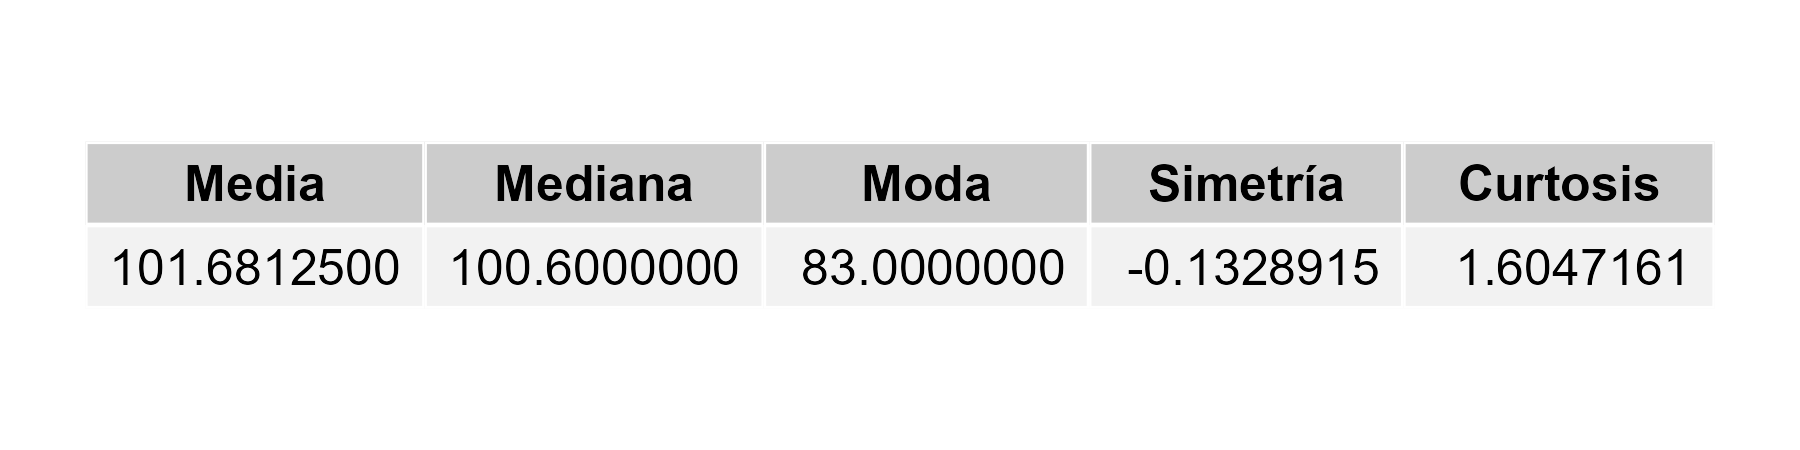
\includegraphics[width=\textwidth]{MTC/GNP.deflator_central.png}
            \caption{Medidas de Tendencia Central para GNP.deflator}
        \end{figure}
        \begin{figure}[H]
            \centering
            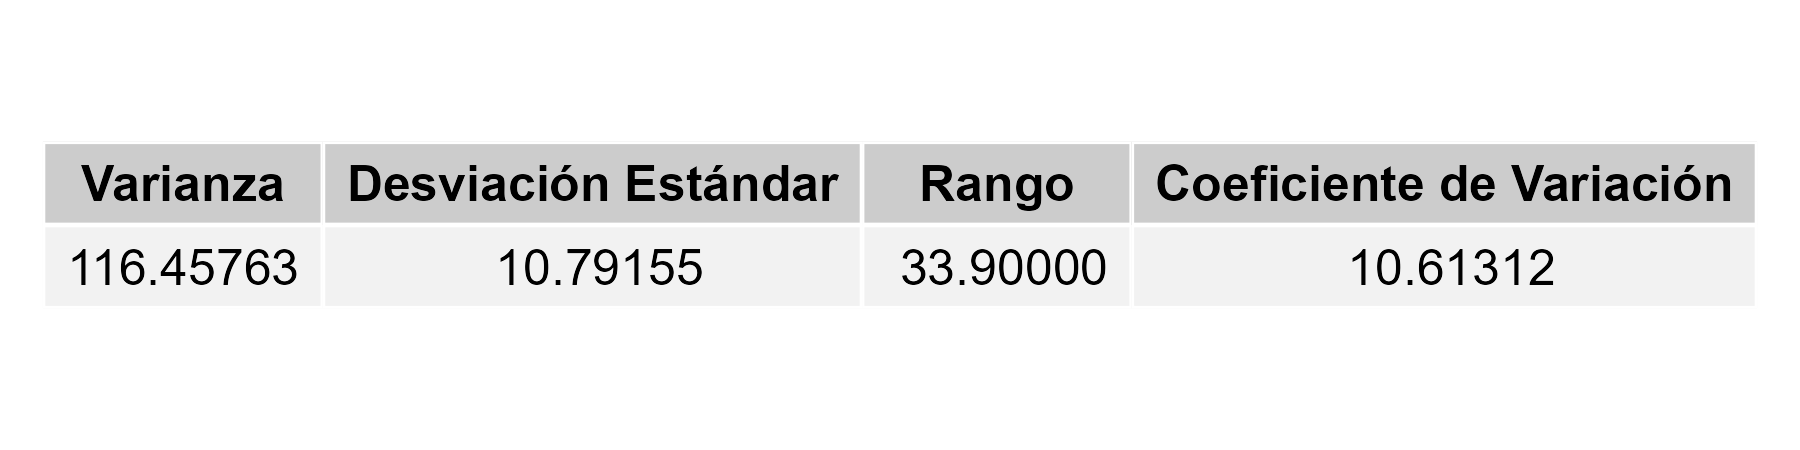
\includegraphics[width=\textwidth]{MTC/GNP.deflator_dispersion.png}
            \caption{Medidas de Dispersión para GNP.deflator}
        \end{figure}
            \begin{itemize}
                \item La media es 101.68, indicando el nivel promedio del deflactor del PNB.
                \item La mediana es 100.6, lo que sugiere que la mitad de los valores están por debajo de este nivel.
                \item La moda es 83, el valor más frecuente.
                \item La simetría negativa (-0.13) sugiere una ligera inclinación hacia la izquierda.
                \item La curtosis de 1.60 indica que la distribución es algo más plana que una distribución normal.
                \item La varianza es 116.46, reflejando la dispersión de los datos.
                \item La desviación estándar es 10.79, lo que muestra la variabilidad promedio respecto a la media.
                \item El rango es 33.9, lo que refleja la diferencia entre el valor más alto y el más bajo.
                \item El coeficiente de variación es 10.61%, indicando una variabilidad moderada relativa a la media.
            \end{itemize}
    \end{itemize}

    \begin{figure}[H]
        \centering
        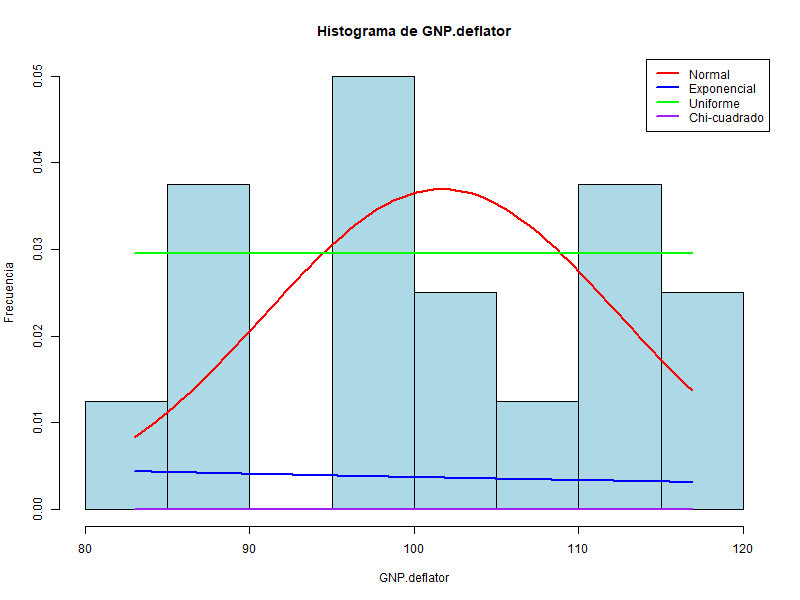
\includegraphics[width=0.5\textwidth]{HistogramasDensidad/histograma_GNP.deflator.png}
        \caption{Histograma y curvas de densidad para GNP.deflator}
        \vspace{0.5cm}
    \end{figure}

    
    \section{Interpretación de los Resultados} \begin{itemize}
        \item La distribución normal es una buena aproximación para el Producto Nacional Bruto (GNP) del conjunto de datos Longley, lo que significa que la mayoría de los valores se concentran alrededor de un valor central (la media) y disminuyen simétricamente hacia ambos lados.
        \item La media y la desviación estándar son medidas importantes para describir la distribución normal. La media representa el valor central, mientras que la desviación estándar indica la dispersión de los datos alrededor de la media.
        \item La simetría y unimodalidad del histograma sugieren que no hay evidencia de una distribución bimodal o multimodal, lo que podría indicar la presencia de subgrupos distintos en los datos.
        \item La presencia de algunos valores atípicos puede indicar la existencia de observaciones inusuales o extremas en el conjunto de datos, que podrían requerir un análisis más profundo.
        \end{itemize}
    
    
    \item \textbf{GNP (Gross National Product)}
    \begin{itemize}
        \item \textbf{Descripción:} Producto Nacional Bruto en millones de dólares.
        \item \textbf{Escala:} Cuantitativa Continua.
        \item \textbf{Significado:} Mide el valor total de los bienes y servicios producidos por la economía de un país, incluyendo los ingresos del extranjero. Indica la salud económica general.
        \item \textbf{Análisis:} 
        \begin{figure}[H]
            \centering
            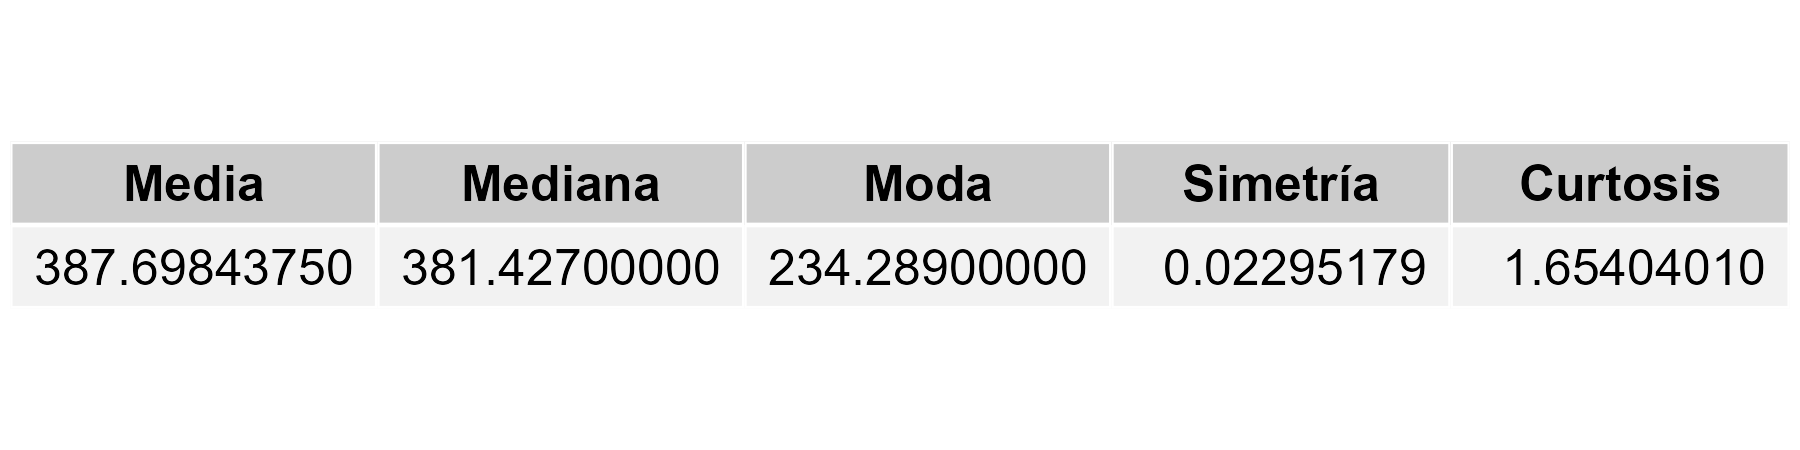
\includegraphics[width=\textwidth]{MTC/GNP_central.png}
            \caption{Medidas de Tendencia Central para GNP}
        \end{figure}
        \begin{figure}[H]
            \centering
            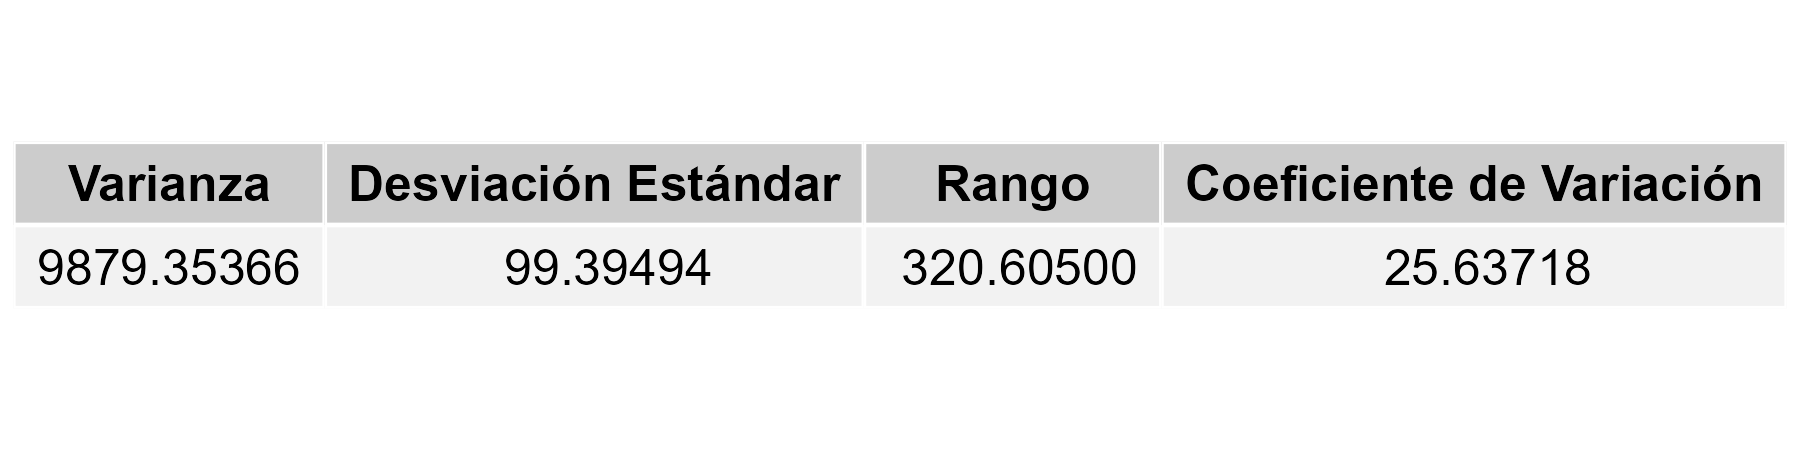
\includegraphics[width=\textwidth]{MTC/GNP_dispersion.png}
            \caption{Medidas de Dispersión para GNP}
        \end{figure}
            \begin{itemize}
                \item La media es 387.70, indicando el promedio del PNB.
                \item La mediana es 381.43, lo que sugiere que la mitad de los valores están por debajo de este nivel.
                \item La moda es 234.29, el valor más frecuente.
                \item La simetría positiva (0.02) sugiere una ligera inclinación hacia la derecha.
                \item La curtosis de 1.65 indica una distribución algo más apuntada que una distribución normal.
                \item La varianza es 9879.35, reflejando una alta dispersión de los datos.
                \item La desviación estándar es 99.39, mostrando una gran variabilidad promedio respecto a la media.
                \item El rango es 320.61, reflejando una gran diferencia entre el valor más alto y el más bajo.
                \item El coeficiente de variación es 25.64%, indicando una variabilidad significativa relativa a la media.
            \end{itemize}
    \end{itemize}
    
    \begin{figure}[H]
        \centering
        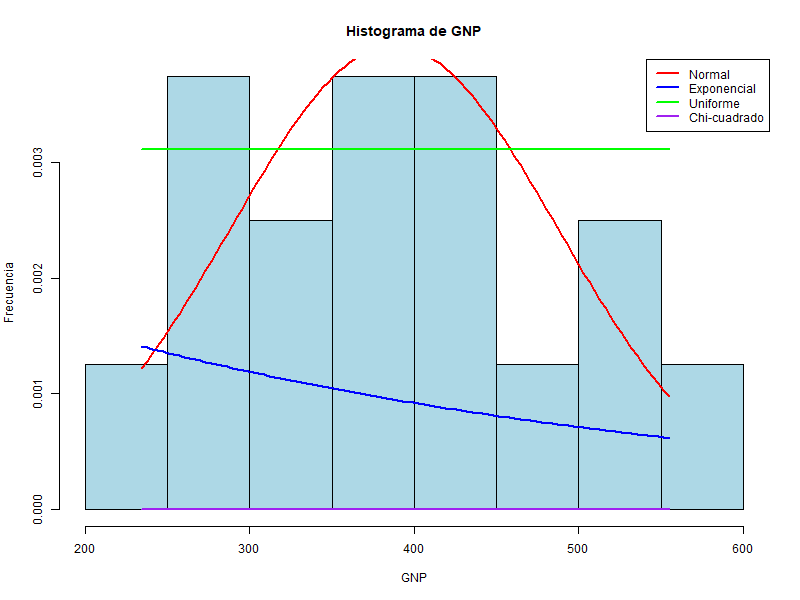
\includegraphics[width=0.5\textwidth]{HistogramasDensidad/histograma_GNP.png}
        \caption{Histograma y curvas de densidad para GNP}
        \vspace{0.5cm}
    \end{figure}

    \item \textbf{Unemployed}
    \begin{itemize}
        \item \textbf{Descripción:} Número de personas desempleadas en miles.
        \item \textbf{Escala:} Cuantitativa Continua.
        \item \textbf{Significado:} Representa la cantidad de personas en la fuerza laboral que están buscando trabajo pero no tienen empleo.
        \item \textbf{Análisis:} 
        \begin{figure}[H]
            \centering
            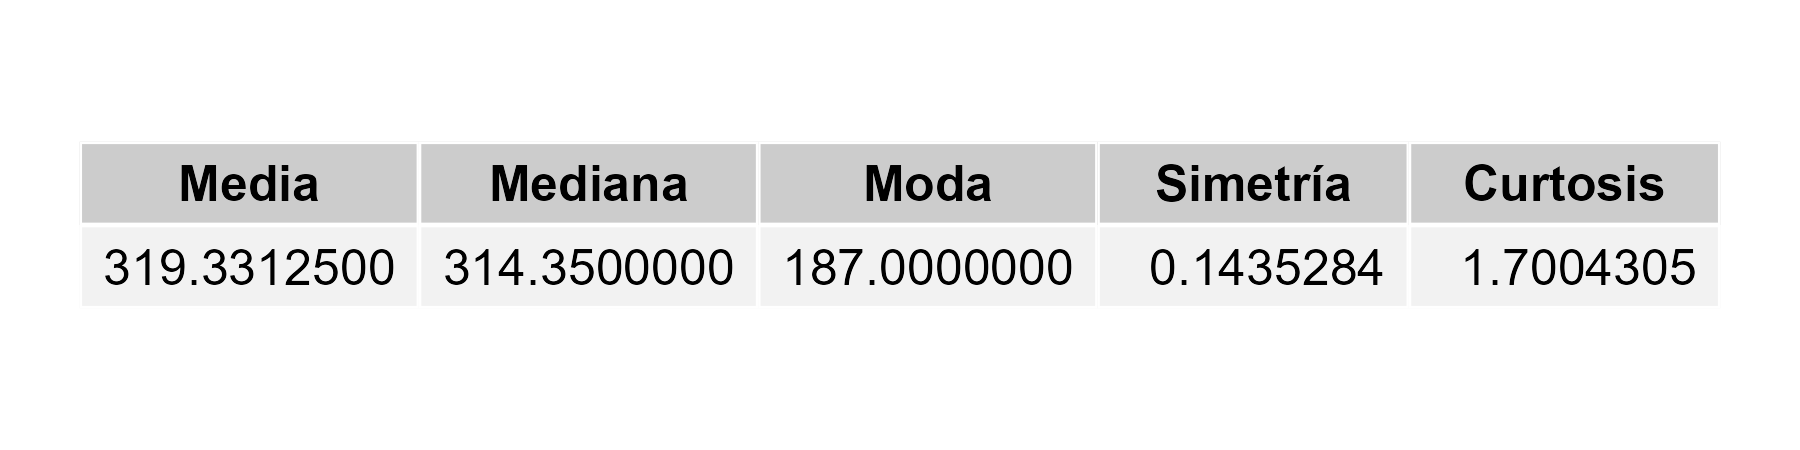
\includegraphics[width=\textwidth]{MTC/Unemployed_central.png}
            \caption{Medidas de Tendencia Central para Unemployed}
        \end{figure}
        \begin{figure}[H]
            \centering
            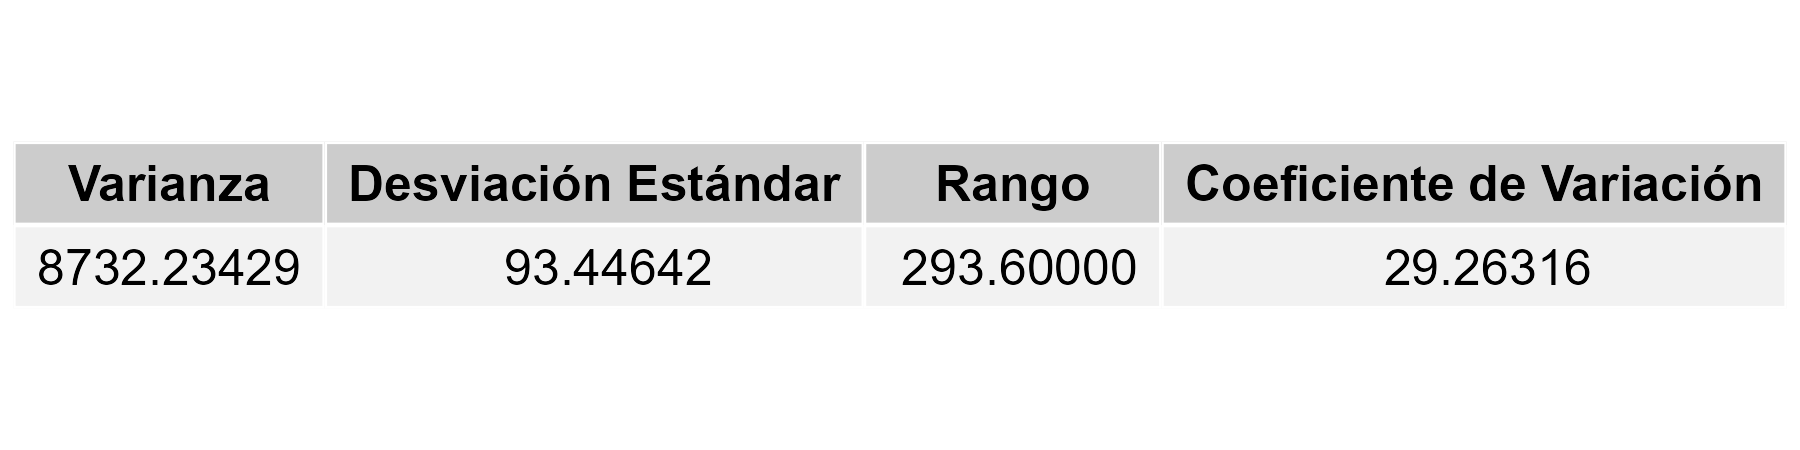
\includegraphics[width=\textwidth]{MTC/Unemployed_dispersion.png}
            \caption{Medidas de Dispersión para Unemployed}
        \end{figure}
            \begin{itemize}
                \item La media es 319.33, indicando el promedio de personas desempleadas.
                \item La mediana es 314.35, lo que sugiere que la mitad de los valores están por debajo de este nivel.
                \item La moda es 187, el valor más frecuente.
                \item La simetría positiva (0.14) sugiere una ligera inclinación hacia la derecha.
                \item La curtosis de 1.70 indica una distribución algo más apuntada que una distribución normal.
                \item La varianza es 8732.23, reflejando una alta dispersión de los datos.
                \item La desviación estándar es 93.45, mostrando una gran variabilidad promedio respecto a la media.
                \item El rango es 293.6, lo que refleja una gran diferencia entre el valor más alto y el más bajo.
                \item El coeficiente de variación es 29.26%, indicando una alta variabilidad relativa a la media.
            \end{itemize}
    \end{itemize}

    \begin{figure}[H]
        \centering
        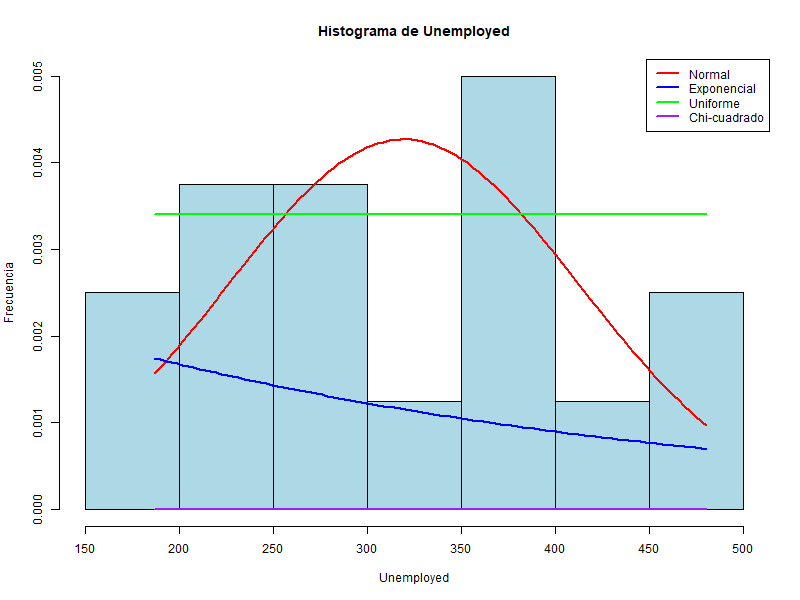
\includegraphics[width=0.5\textwidth]{HistogramasDensidad/histograma_Unemployed.png}
        \caption{Histograma y curvas de densidad para Unemployed}
        \vspace{0.5cm}
    \end{figure}
    
    \item \textbf{Armed.Forces}
    \begin{itemize}
        \item \textbf{Descripción:} Número de personas enlistadas en las fuerzas armadas en miles.
        \item \textbf{Escala:} Cuantitativa Continua.
        \item \textbf{Significado:} Indica el tamaño de la fuerza laboral militar activa en la economía.
        \item \textbf{Análisis:} 
        \begin{figure}[H]
            \centering
            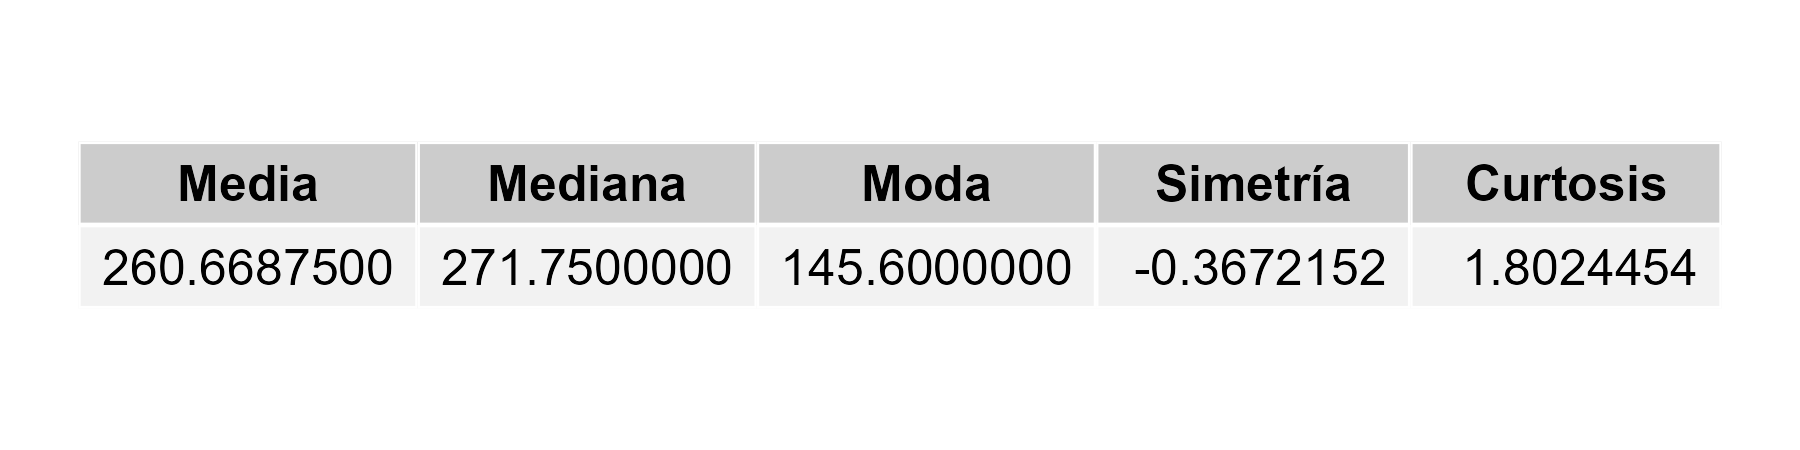
\includegraphics[width=\textwidth]{MTC/Armed.Forces_central.png}
            \caption{Medidas de Tendencia Central para Armed.Forces}
        \end{figure}
        \begin{figure}[H]
            \centering
            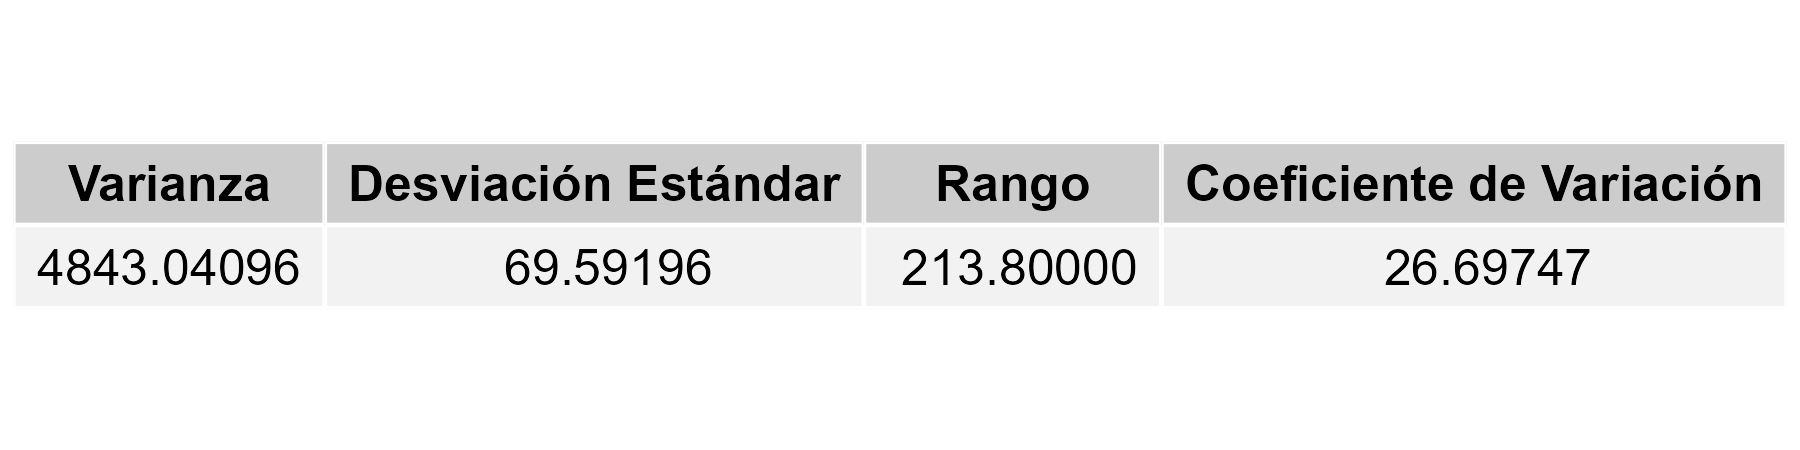
\includegraphics[width=\textwidth]{MTC/Armed.Forces_dispersion.png}
            \caption{Medidas de Dispersión para Armed.Forces}
        \end{figure}
            \begin{itemize}
                \item La media es 260.67, indicando el promedio de personal militar.
                \item La mediana es 271.75, lo que sugiere que la mitad de los valores están por debajo de este nivel.
                \item La moda es 145.6, el valor más frecuente.
                \item La simetría negativa (-0.37) sugiere una inclinación hacia la izquierda.
                \item La curtosis de 1.80 indica una distribución más apuntada que una distribución normal.
                \item La varianza es 4843.04, reflejando una considerable dispersión de los datos.
                \item La desviación estándar es 69.59, mostrando una variabilidad moderada respecto a la media.
                \item El rango es 213.8, lo que refleja una considerable diferencia entre el valor más alto y el más bajo.
                \item El coeficiente de variación es 26.70%, indicando una alta variabilidad relativa a la media.
            \end{itemize}
    \end{itemize}
    \begin{figure}[H]
        \centering
        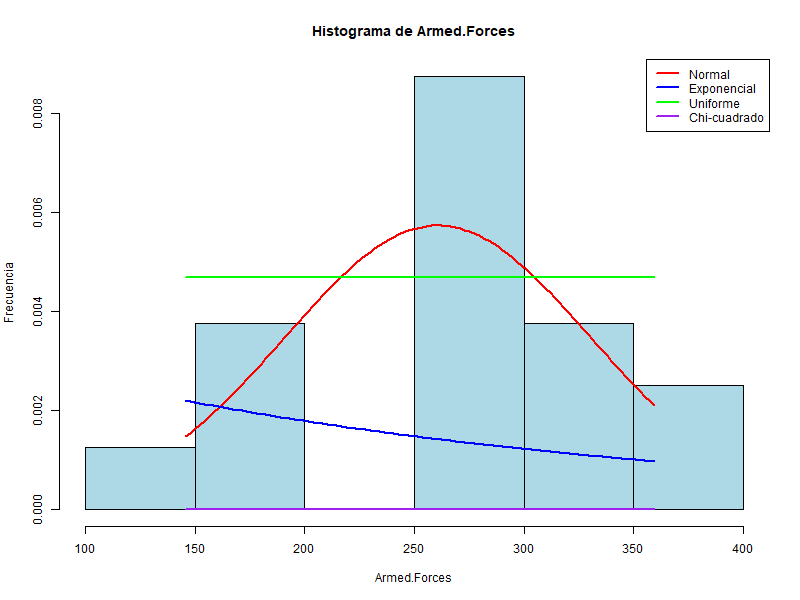
\includegraphics[width=0.5\textwidth]{HistogramasDensidad/histograma_Armed.Forces.png}
        \caption{Histograma y curvas de densidad para Armed Forces}
        \vspace{0.5cm}
    \end{figure}

    \item \textbf{Population}
    \begin{itemize}
        \item \textbf{Descripción:} Tamaño de la población en miles.
        \item \textbf{Escala:} Cuantitativa Continua.
        \item \textbf{Significado:} Refleja el tamaño total de la población en un determinado año. Es un indicador demográfico que puede influir en variables económicas.
        \item \textbf{Análisis:} 
        \begin{figure}[H]
            \centering
            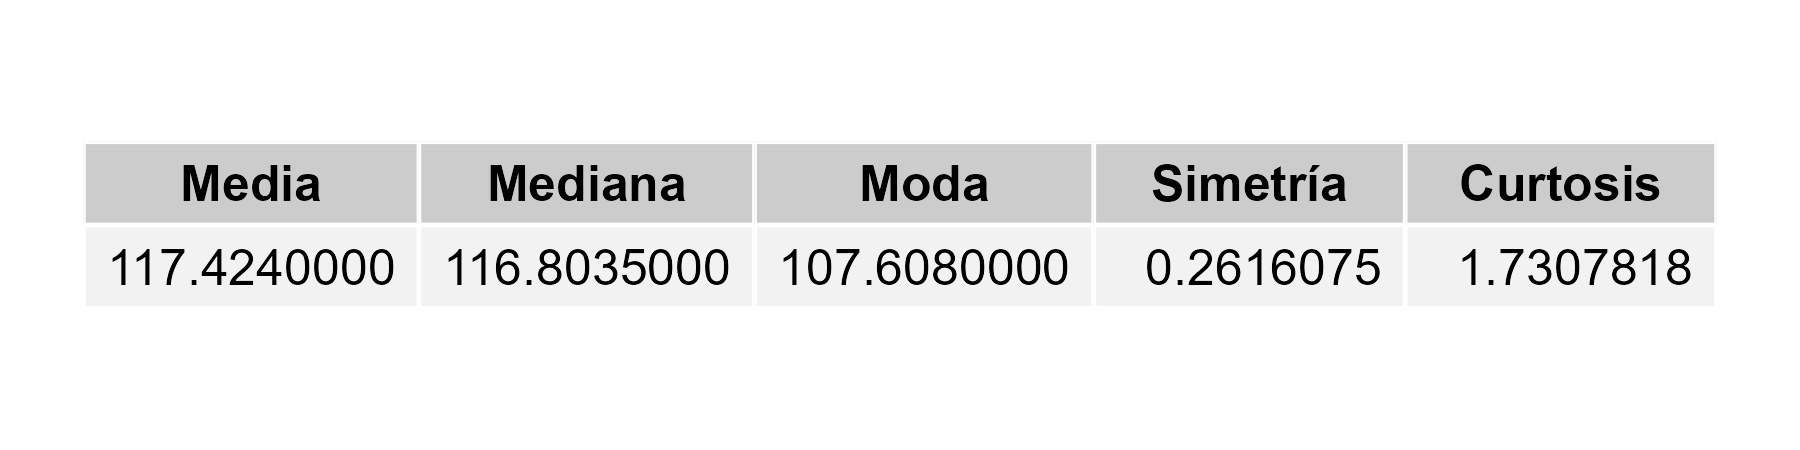
\includegraphics[width=\textwidth]{MTC/Population_central.png}
            \caption{Medidas de Tendencia Central para Population}
        \end{figure}
        \begin{figure}[H]
            \centering
            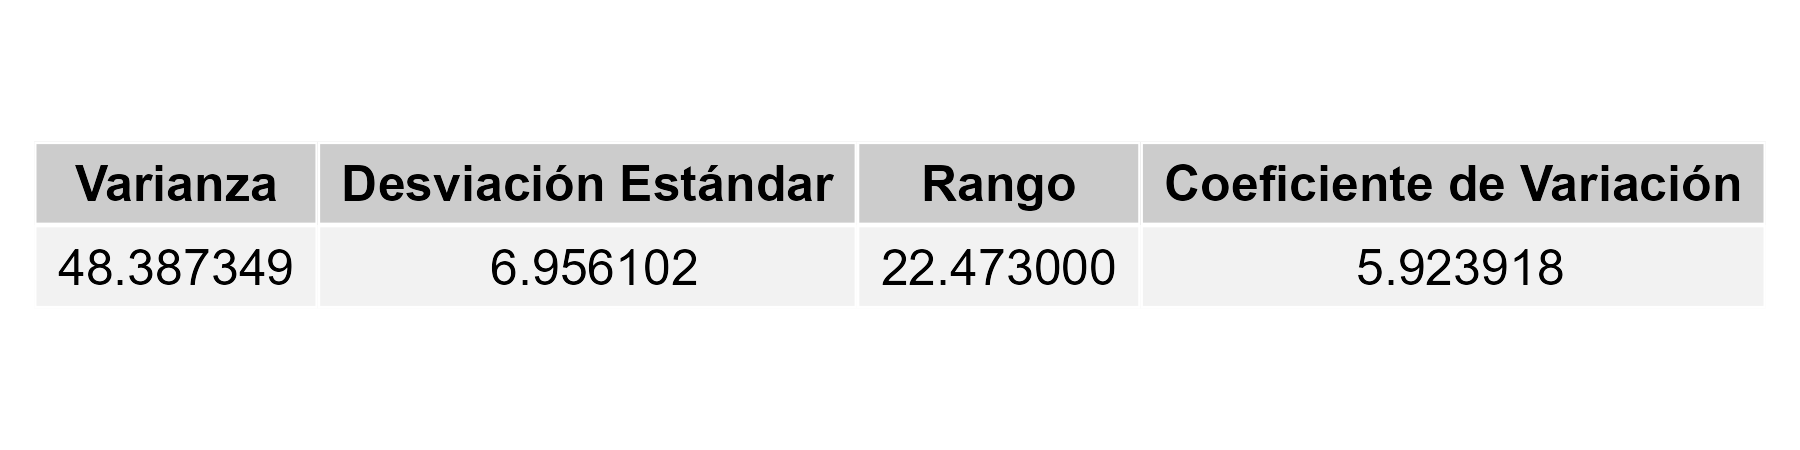
\includegraphics[width=\textwidth]{MTC/Population_dispersion.png}
            \caption{Medidas de Dispersión para Population}
        \end{figure}
            \begin{itemize}
                \item La media es 117.42, indicando el tamaño promedio de la población.
                \item La mediana es 116.80, lo que sugiere que la mitad de los valores están por debajo de este nivel.
                \item La moda es 107.61, el valor más frecuente.
                \item La simetría positiva (0.26) sugiere una inclinación hacia la derecha.
                \item La curtosis de 1.73 indica una distribución algo más apuntada que una distribución normal.
                \item La varianza es 48.39, reflejando una baja dispersión de los datos.
                \item La desviación estándar es 6.96, mostrando una baja variabilidad respecto a la media.
                \item El rango es 22.47, lo que refleja una diferencia moderada entre el valor más alto y el más bajo.
                \item El coeficiente de variación es 5.92%, indicando una baja variabilidad relativa a la media.
            \end{itemize}
    \end{itemize}
    
    \begin{figure}[H]
        \centering
        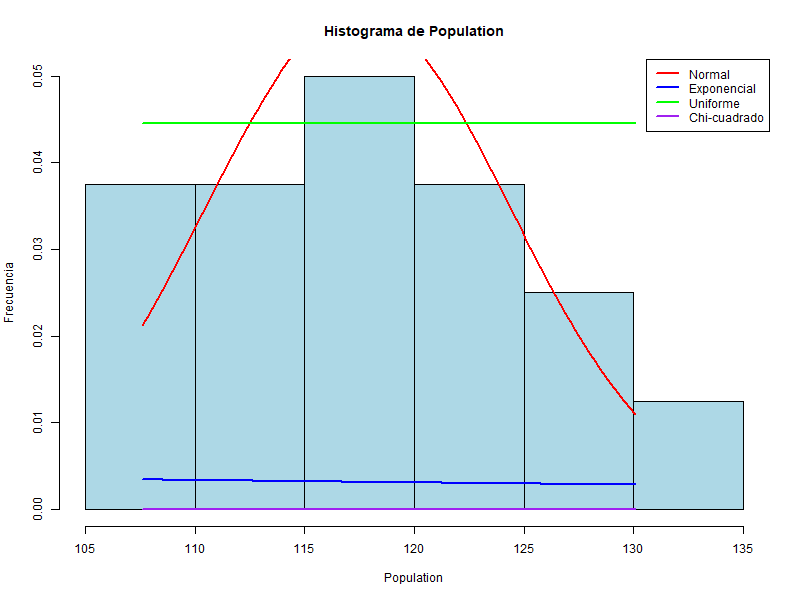
\includegraphics[width=0.5\textwidth]{HistogramasDensidad/histograma_Population.png}
        \caption{Histograma y curvas de densidad para Population}
        \vspace{0.5cm}
    \end{figure}


    \item \textbf{Year}
    \begin{itemize}
        \item \textbf{Descripción:} Año en que se recolectaron los datos.
        \item \textbf{Escala:} Cuantitativa Discreta.
        \item \textbf{Significado:} Indica el año calendario de cada observación.
        \item \textbf{Análisis:} 
    \end{itemize}
    \begin{figure}[H]
        \centering
        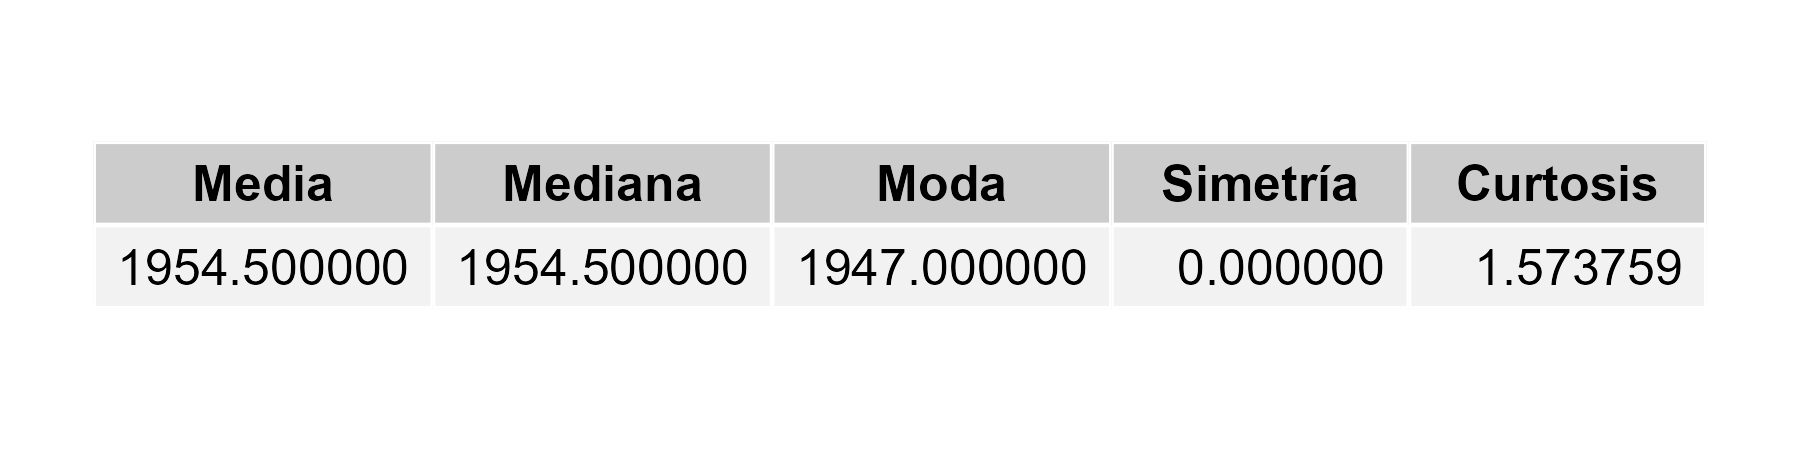
\includegraphics[width=\textwidth]{MTC/Year_central.png}
        \caption{Medidas de Tendencia Central para Year}
    \end{figure}
    \begin{figure}[H]
        \centering
        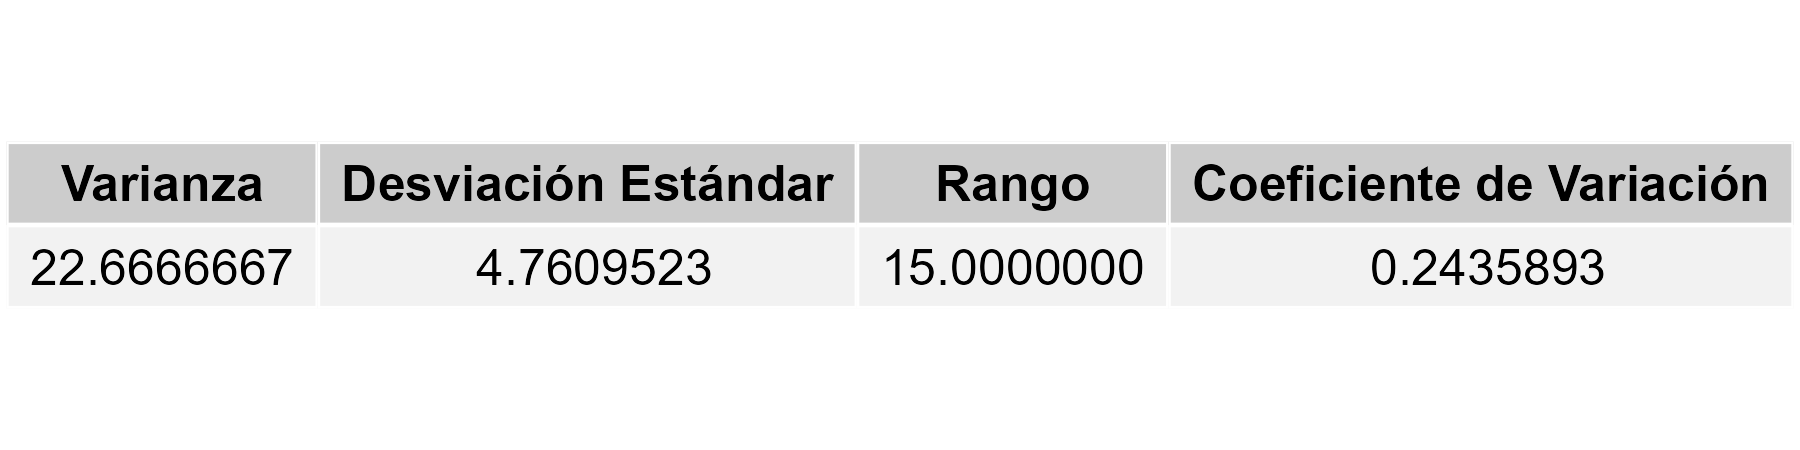
\includegraphics[width=\textwidth]{MTC/Year_dispersion.png}
        \caption{Medidas de Dispersión para Year}
    \end{figure}
            \begin{itemize}
                \item La media es 1954.5, que representa el punto medio del período analizado.
                \item La mediana es 1954.5, coincidiendo con la media, lo que sugiere una distribución simétrica.
                \item La moda es 1947, el valor más frecuente.
                \item La simetría es 0, indicando que la distribución es simétrica.
                \item La curtosis de 1.57 indica que la distribución es algo más plana que una distribución normal.
                \item La varianza es 22.67, lo que refleja una baja dispersión de los datos.
                \item La desviación estándar es 4.76, mostrando una baja variabilidad respecto a la media.
                \item El rango es 15, lo que refleja una diferencia moderada entre el valor más alto y el más bajo.
                \item El coeficiente de variación es 0.24%, indicando una muy baja variabilidad relativa a la media.
            \end{itemize}
    
            \begin{figure}[H]
                \centering
                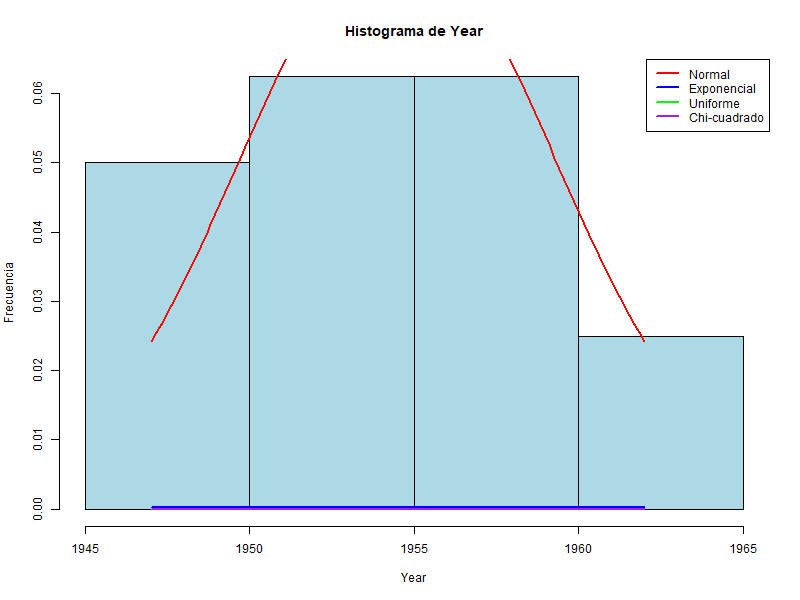
\includegraphics[width=0.5\textwidth]{HistogramasDensidad/histograma_Year.png}
                \caption{Histograma y curvas de densidad para Year}
                \vspace{0.5cm}
            \end{figure}

    \item \textbf{Employed}
    \begin{itemize}
        \item \textbf{Descripción:} Número de personas empleadas en miles.
        \item \textbf{Escala:} Cuantitativa Continua.
        \item \textbf{Significado:} Representa la cantidad de personas con empleo en la fuerza laboral.
        \item \textbf{Análisis:} 
    \end{itemize}
    \begin{figure}[H]
        \centering
        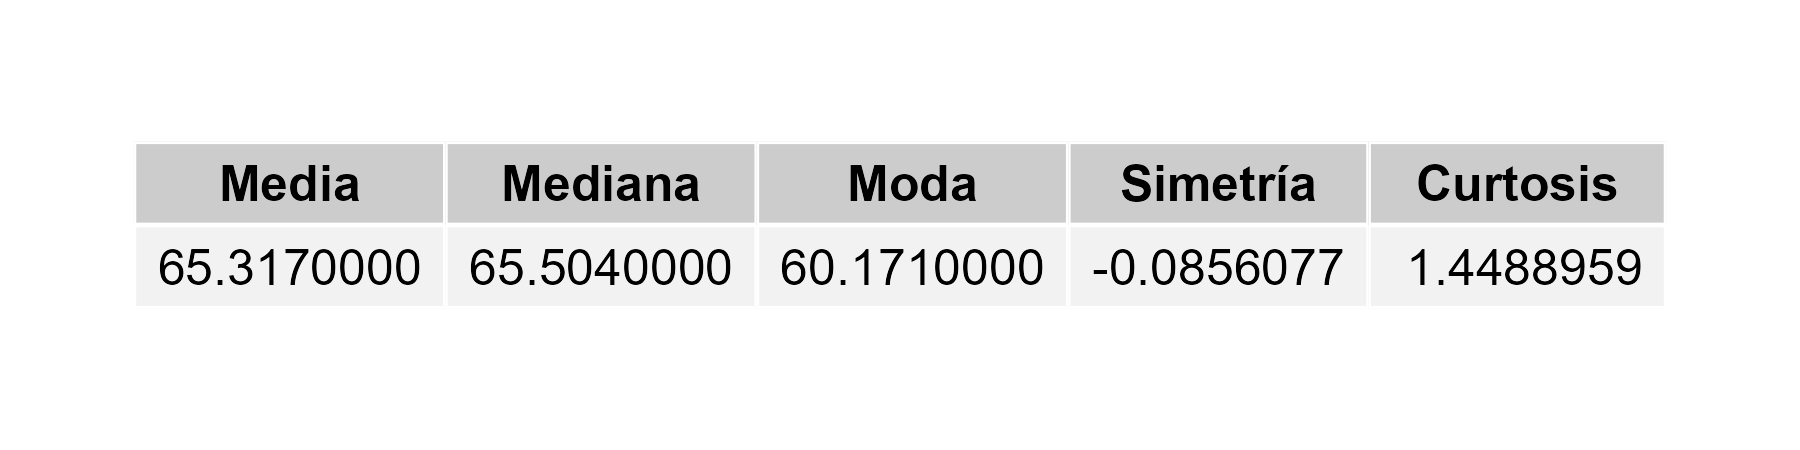
\includegraphics[width=\textwidth]{MTC/Employed_central.png}
        \caption{Medidas de Tendencia Central para Employed}
    \end{figure}
    \begin{figure}[H]
        \centering
        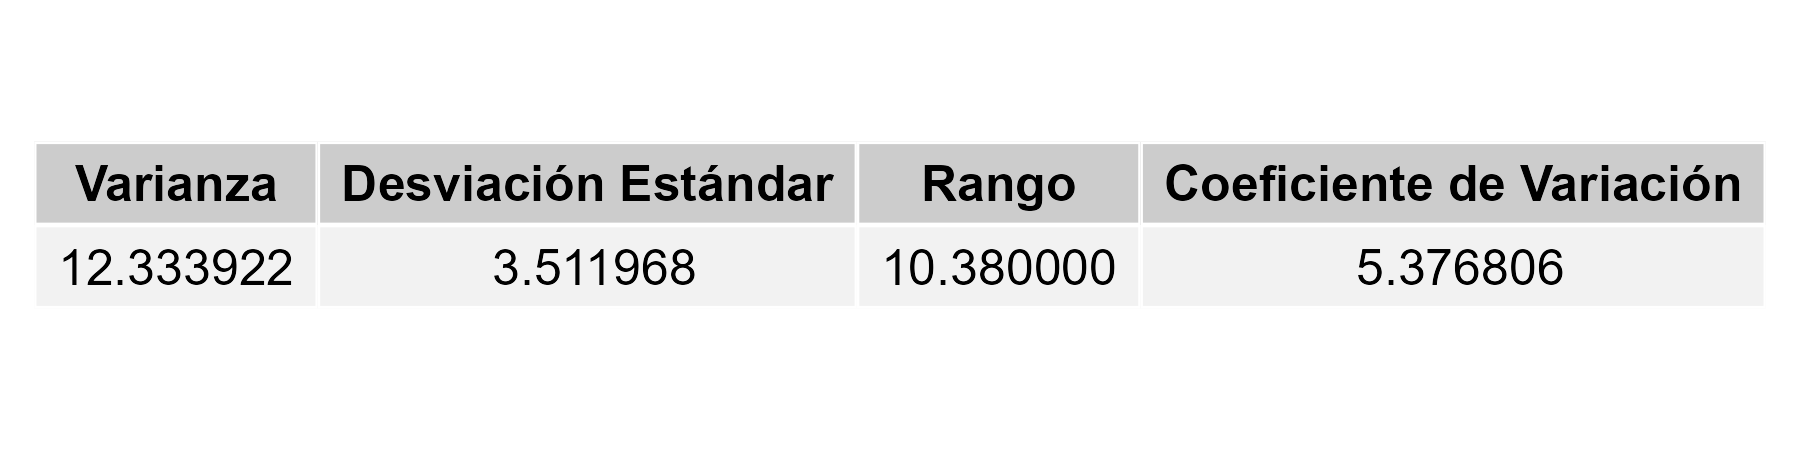
\includegraphics[width=\textwidth]{MTC/Employed_dispersion.png}
        \caption{Medidas de Dispersión para Employed}
    \end{figure}
            \begin{itemize}
                \item La media es 65.32, indicando el promedio de personas empleadas.
                \item La mediana es 65.50, lo que sugiere que la mitad de los valores están por debajo de este nivel.
                \item La moda es 60.17, el valor más frecuente.
                \item La simetría negativa (-0.09) sugiere una ligera inclinación hacia la izquierda.
                \item La curtosis de 1.45 indica que la distribución es más plana que una distribución normal.
                \item La varianza es 12.33, lo que refleja una baja dispersión de los datos.
                \item La desviación estándar es 3.51, mostrando una baja variabilidad respecto a la media.
                \item El rango es 10.38, lo que refleja una diferencia moderada entre el valor más alto y el más bajo.
                \item El coeficiente de variación es 5.38%, indicando una baja variabilidad relativa a la media.
            \end{itemize}
\end{itemize}

\begin{figure}[H]
    \centering
    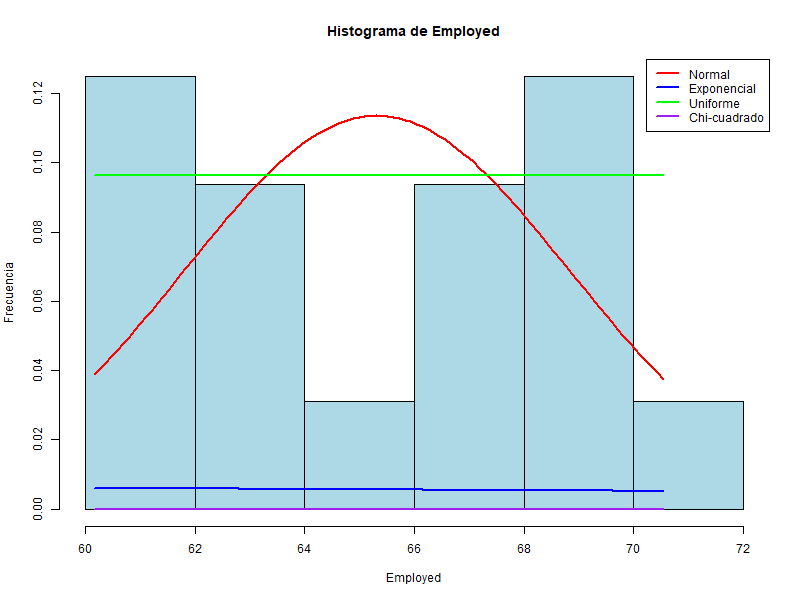
\includegraphics[width=0.5\textwidth]{HistogramasDensidad/histograma_Employed.png}
    \caption{Histograma y curvas de densidad para Employed}
    \vspace{0.5cm}
\end{figure}

\section{Análisis de la Matriz de Correlación}


\begin{table}[ht]
    \centering
    \begin{adjustbox}{max width=\textwidth}
    \begin{tabular}{lrrrrrrr}
    \hline
     & GNP.deflator & GNP & Unemployed & Armed.Forces & Population & Year & Employed \\ 
    \hline
    GNP.deflator & 1.00 & 0.99 & 0.62 & 0.46 & 0.98 & 0.99 & 0.97 \\ 
    GNP & 0.99 & 1.00 & 0.60 & 0.45 & 0.99 & 1.00 & 0.98 \\ 
    Unemployed & 0.62 & 0.60 & 1.00 & -0.18 & 0.69 & 0.67 & 0.50 \\ 
    Armed.Forces & 0.46 & 0.45 & -0.18 & 1.00 & 0.36 & 0.42 & 0.46 \\ 
    Population & 0.98 & 0.99 & 0.69 & 0.36 & 1.00 & 0.99 & 0.96 \\ 
    Year & 0.99 & 1.00 & 0.67 & 0.42 & 0.99 & 1.00 & 0.97 \\ 
    Employed & 0.97 & 0.98 & 0.50 & 0.46 & 0.96 & 0.97 & 1.00 \\ 
    \hline
    \end{tabular}
    \end{adjustbox}
    \caption{Correlation Matrix of the Longley Dataset}
    \label{tab:correlation_matrix_longley}
    \end{table}
    
    \begin{figure}[h] % 'h' indica que la imagen debe aparecer aquí
        \centering % Centra la imagen
        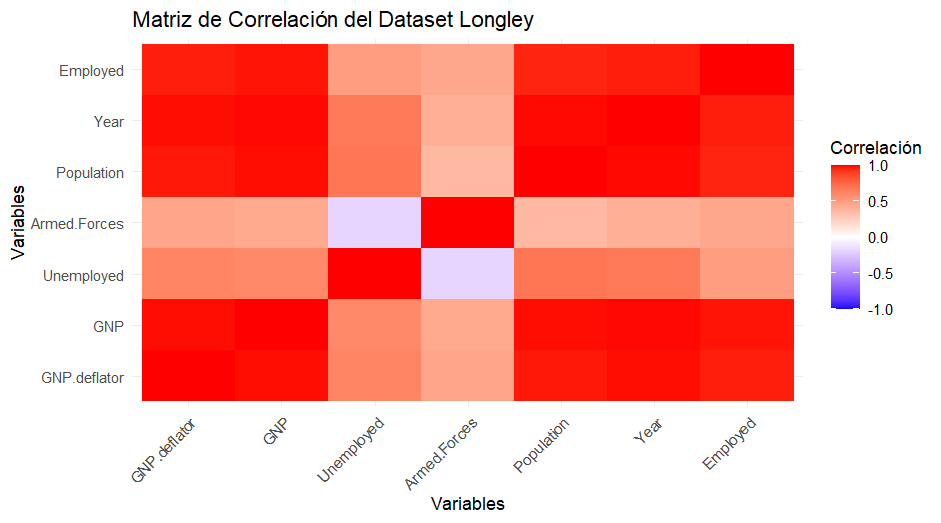
\includegraphics[width=0.5\textwidth]{Correlacion.png}
        \caption{Grafico de Calor , Correlaciones } % Título de la figura
        \label{fig:mi_imagen} % Etiqueta para referencias cruzadas
        \vspace{0.5cm} % Espacio entre las imágenes
    \end{figure}

    \section{Análisis de Correlaciones}

    \subsection{Correlaciones Fuertes Positivas}
    
    \begin{itemize}
        \item \textbf{GNP.deflator y GNP: 0.99} \\
        Esta correlación muy fuerte indica que a medida que el deflactor del PNB (GNP.deflator) aumenta, el PNB también tiende a aumentar. Este resultado es coherente con las expectativas en economía, donde un aumento en el PNB generalmente se asocia con un aumento en los precios y, por lo tanto, en el deflactor del PNB.
        
        \begin{figure}[H]
            \centering
            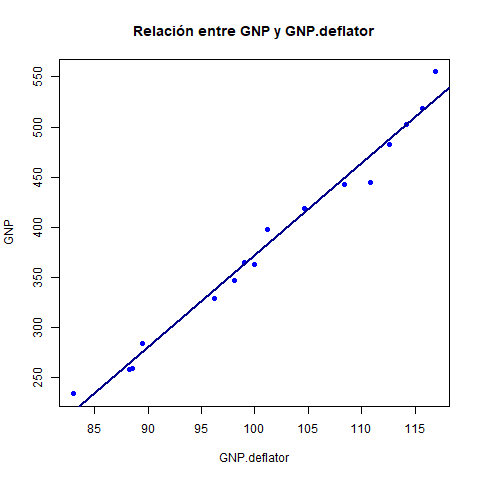
\includegraphics[width=0.5\textwidth]{GraficosDispersion/GNP.deflator_vs_GNP.png}
            \label{fig:GNP.deflator_vs_GNP}
            \vspace{0.5cm} % Espacio entre las imágenes
        \end{figure}
           

        \item \textbf{GNP y Year: 1.00} \\
        La correlación perfecta entre GNP y el Año sugiere que el PNB ha aumentado de manera constante con el tiempo en el periodo estudiado. Esto podría reflejar un crecimiento económico constante durante los años observados.
        
        \begin{figure}[H]
            \centering
            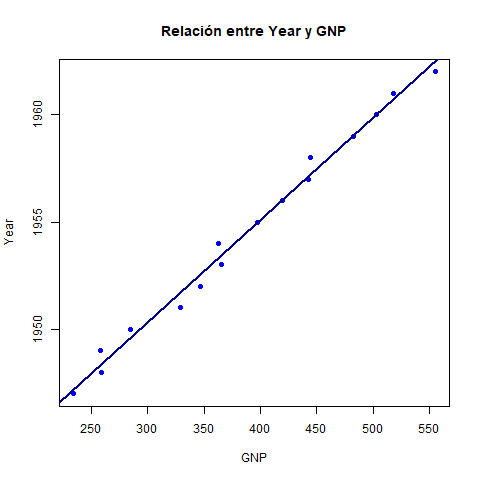
\includegraphics[width=0.5\textwidth]{GraficosDispersion/GNP_vs_Year.png}
            \label{fig:GNP_vs_Year}
            \vspace{0.5cm} % Espacio entre las imágenes
        \end{figure}

        \item \textbf{Population y GNP: 0.99} \\
        Esta correlación muy alta sugiere que a medida que la población aumenta, también lo hace el PNB. Esto podría indicar que el crecimiento económico ha ido de la mano con el crecimiento poblacional.
    
                
        \begin{figure}[H]
            \centering
            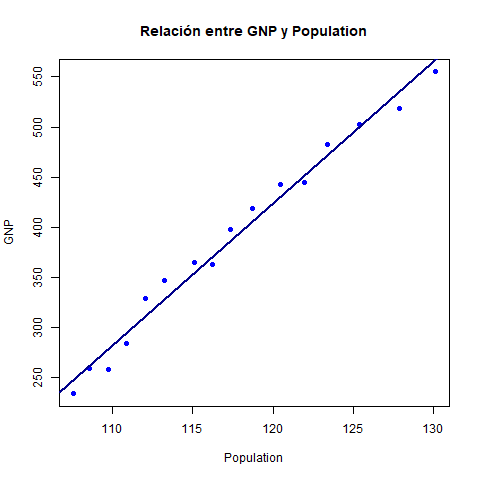
\includegraphics[width=0.5\textwidth]{GraficosDispersion/Population_vs_GNP.png}
            \label{fig:Population_vs_GNP}
            \vspace{0.5cm} % Espacio entre las imágenes
        \end{figure}
    
    \end{itemize}
    
    \subsection{Correlaciones Fuertes Negativas}
    
    \begin{itemize}
        \item \textbf{No se observan correlaciones fuertes negativas} \\
        En la tabla proporcionada, no se observan correlaciones negativas significativas entre las variables analizadas.
    \end{itemize}
    
    \subsection{Correlaciones Moderadas}
    
    \begin{itemize}
        \item \textbf{Unemployed y Population: 0.69} \\
        Existe una relación moderada entre el número de desempleados y la población total. Esto podría indicar que a medida que la población crece, el número absoluto de desempleados también tiende a aumentar, aunque no necesariamente a la misma tasa.
        
        \item \textbf{Armed.Forces y Year: 0.42} \\
        Esta correlación moderada sugiere una ligera tendencia a que, con el paso del tiempo, las Fuerzas Armadas han variado de manera no tan directa con los otros factores, lo cual podría reflejar cambios en políticas de defensa o en la situación geopolítica.
    \end{itemize}
    
    \subsection{Correlaciones Débiles}
    
    \begin{itemize}
        \item \textbf{Armed.Forces y Unemployed: -0.18} \\
        La correlación negativa débil entre las Fuerzas Armadas y el desempleo indica que no hay una relación clara y fuerte entre estos dos factores. Esto podría reflejar que el tamaño de las Fuerzas Armadas no está directamente influenciado por los niveles de desempleo.
    \end{itemize}

    \section*{Análisis del Modelo de Regresión Lineal: \texttt{GNP.deflator ~ GNP}}

\subsection*{Resumen del Modelo}

\textbf{Call:}  
El modelo de regresión lineal fue ajustado con la fórmula \texttt{longley\$GNP.deflator ~ longley\$GNP}, donde \texttt{GNP.deflator} es la variable dependiente y \texttt{GNP} es la variable independiente.

\subsection*{Residuos}
Los residuos del modelo, que representan las diferencias entre los valores observados y los valores predichos, se distribuyen de la siguiente manera:
\begin{itemize}
    \item \textbf{Mínimo}: -2.7814
    \item \textbf{1er Cuartil (1Q)}: -0.6233
    \item \textbf{Mediana}: 0.3123
    \item \textbf{3er Cuartil (3Q)}: 0.7925
    \item \textbf{Máximo}: 2.9986
\end{itemize}

Esto indica que la mayoría de los errores de predicción están relativamente cerca de cero, lo que sugiere un buen ajuste del modelo.

\subsection*{Coeficientes}
El modelo proporciona los siguientes coeficientes para la ecuación de regresión:

\begin{itemize}
    \item \textbf{Intercepto}: 59.941915  
    Este es el valor estimado de \texttt{GNP.deflator} cuando \texttt{GNP} es cero. Aunque un valor de \texttt{GNP} igual a cero no es realista, este valor tiene sentido en el contexto del modelo.

    \item \textbf{longley\$GNP}: 0.107659  
    Este coeficiente indica que por cada aumento de una unidad en \texttt{GNP}, el \texttt{GNP.deflator} aumenta en aproximadamente 0.107659 unidades. Dado que el coeficiente es positivo, esto sugiere una relación directa entre \texttt{GNP} y \texttt{GNP.deflator}, donde a medida que aumenta el \texttt{GNP}, también lo hace el \texttt{GNP.deflator}.
\end{itemize}

\subsection*{Significancia Estadística}
\begin{itemize}
    \item \textbf{Valor t del intercepto}: 39.96  
    \item \textbf{Valor t del coeficiente de GNP}: 28.67  
    \item \textbf{p-valor del intercepto}: 7.89e-16  
    \item \textbf{p-valor del coeficiente de GNP}: 7.81e-14  
\end{itemize}

Ambos p-valores son extremadamente pequeños (mucho menores que 0.001), lo que indica que tanto el intercepto como el coeficiente de \texttt{GNP} son altamente significativos. Esto significa que \texttt{GNP} es una variable relevante para predecir \texttt{GNP.deflator}.

\subsection*{Estadísticas del Modelo}
\begin{itemize}
    \item \textbf{Error estándar residual}: 1.446  
    Este valor mide la dispersión de los residuos y sugiere que, en promedio, las predicciones del modelo tienen un error de $\pm1.446$ unidades.

    \item \textbf{R-cuadrado múltiple}: 0.9832  
    Este valor indica que el modelo explica el 98.32\% de la variabilidad observada en \texttt{GNP.deflator}, lo que sugiere un ajuste excelente del modelo.

    \item \textbf{R-cuadrado ajustado}: 0.9821  
    Este valor ajusta el R-cuadrado por el número de predictores en el modelo, confirmando que el modelo sigue siendo muy fuerte incluso después de tener en cuenta el ajuste.

    \item \textbf{F-Estadístico}: 821.8  
    Este valor, junto con un p-valor extremadamente pequeño (7.809e-14), indica que el modelo es globalmente significativo, lo que significa que hay una relación estadísticamente significativa entre \texttt{GNP} y \texttt{GNP.deflator}.
\end{itemize}

\subsection*{Conclusión}
El modelo de regresión lineal \texttt{GNP.deflator ~ GNP} muestra una fuerte relación positiva entre \texttt{GNP} y \texttt{GNP.deflator}, donde un aumento en el \texttt{GNP} está asociado con un aumento en el \texttt{GNP.deflator}. Dado el alto valor de R-cuadrado y la significancia estadística de los coeficientes, el modelo es muy confiable para predecir \texttt{GNP.deflator} en función de \texttt{GNP}.

\end{document}
